\section{"3" Оптимизация кинематической схемы}

\begin{frame}[t]{Определение количества ног}
    \framesubtitle{}
    \begin{columns}[T,onlytextwidth]
        \begin{column}{0.59\textwidth}
            \small
            Решить $F=f(x) \rightarrow max$ критерий оптимизации, где

            $f(x)$ --- \textbf{ Критерии}: пройденная дистанция, длина корпуса\\
            $(x)$ --- \textbf{Параметры}: количество ног, сдвиг фазы между
            соседними ногами

            \textbf{Метод решения}: Генетический алгоритм: Open AI-ES

            \textbf{Идея решения}: генерируется множество особей, а
            также семейство территорий с одинаковой сложностью.
            За фиксированное время, с постоянной угловой скоростью
            на моторах, каждый робот проходит это семейство
            территорий и записываются данные.

            \textbf{Предположения}: 1) есть только сухое трение
            между ногами и поверхностью. 2) Созданные
            поверхности с помощью одной функции
            и параметров имеют одинаковую сложность.

            \textbf{Утверждение}:\textit{Количество ног имеет прямую
                зависимость с длиной корпуса робота.}
        \end{column}
        \begin{column}{0.39\textwidth}
            \begin{figure}[H]
                \begin{subfigure}{0.49\textwidth}
                    \centering\includegraphics[height=2cm,width=1\textwidth,keepaspectratio]{../images/terrain_1.jpg}
                    % \caption{capture1}
                \end{subfigure}
                \begin{subfigure}{0.49\textwidth}
                    \centering\includegraphics[height=2cm,width=1\textwidth,keepaspectratio]{../images/terrain_2.jpg}
                    % \caption{capture2}
                \end{subfigure}

                \begin{subfigure}{0.99\textwidth}
                    \centering\includegraphics[height=2.5cm,width=1\textwidth,keepaspectratio]{../images/terrain_3.jpg}
                    \caption*{Пример прохождения особью сгенерированной поверхности}
                \end{subfigure}
            \end{figure}
        \end{column}
    \end{columns}
\end{frame}

\begin{frame}[t]{Целевая функция}
    \framesubtitle{}
    \vspace{-0.4cm}
    \begin{columns}[T,onlytextwidth]
        \begin{column}{0.48\textwidth}
            \begin{eqnarray}
                F \rightarrow max = \beta \left( {\omega}_{1} \cdot \delta + {\omega}_{2} \cdot L\right) + \\ \nonumber + (1 - \beta) {\delta}^{{\omega}_{1}} {\left( L\right)}^{{\omega}_{2}} \\
                L = \frac{1}{(\gamma - 1) h_{\text{leg}}sin(\alpha)}
            \end{eqnarray}
            Где
            $\beta$ -- адаптивный параметр, \\ ${\omega}_{1,2} \in  [ 0..1 ] $ -- весовые коэффициенты, \\
            $\delta$ -- пройденный путь, \\
            $L$ -- упрощенная длина робота

            \textit{Для решения однокритериальной задачи} использовалась аддитивно-мультипликативная свертка
        \end{column}
        \begin{column}{0.50\textwidth}
            \begin{figure}[H]
                \centering
                \centering\includegraphics[height=3cm,width=1\textwidth,keepaspectratio,page=3]{./tikz_pictures.pdf}
            \end{figure}
        \end{column}
    \end{columns}
\end{frame}

\begin{frame}[t]{Описание механической системы}
    \framesubtitle{}
    \begin{align}
        M \dot{\vec{u}} = \vec{g}                                \\
        M = \begin{bmatrix}
                M_1    & \cdots & 0      \\
                \vdots & \ddots & \vdots \\
                0      & \cdots & M_n
            \end{bmatrix},\ M_i = \begin{bmatrix}
                                      m_i E_{3\times 3} & 0   \\
                                      0                 & I_i
                                  \end{bmatrix}        \\
        \vec{u}_i^{\ T} = \begin{bmatrix}
                              \vec{v}_i^{\ T} & \vec{\omega}_i^{\ T}
                          \end{bmatrix} \\
        \vec{g}^{\ T} = \begin{bmatrix}
                            \cdots \  \vec{F}_i^{\ T}, & (\vec{\tau}_i - \vec{\omega}_i \times I_i \vec{\omega}_i)^T\  \cdots
                        \end{bmatrix}
    \end{align}
    где, $M_i$~---~матрицы, содержащие массово-инерционные характеристики; $m_i$~---~масса тела; $I_i$~---~тензор инерции; $\vec{u_i}$~---~вектор обобщённых скоростей; $E$~---~единичная матрица; $\vec{g}$~---~вектор обобщённых сил; $\vec{v_i}$~---~вектор линейной скорости; $\vec{\omega_i}$~---~вектор угловой скорости; $\vec{F_i}$, $\vec{\tau_i}$~---~силы и моменты сил взаимодействия.
\end{frame}

\begin{frame}[t]{Геометрические связи}
    \framesubtitle{}
    Тела соединены цилиндрическими шарнирами:
    \begin{align}
        \phi(q_{j_1},\ u_{j_1},\ \cdots,\ q_{j_k},\ u_{j_k},\ t) \geqslant  0 \\
        \vec{q_i}^{\ T} = \begin{bmatrix}
                              \vec{x}_i^{\ T} & \vec{Q}_i^{\ T}
                          \end{bmatrix}                   \\
        \dot{\vec{q_i}} = \begin{bmatrix}
                              E_{3\times3} & 0            \\
                              0            & G(\vec{q}_i)
                          \end{bmatrix}\vec{u}_i
    \end{align}
    \begin{align}
        \vec{g}_i = \tau_i^T \vec{z}_{i-1} -k_i \dot{\vec{q_i}}
    \end{align}
    где через $\phi$ обозначена функция связи; $t$~---~время; $\vec{q}_{i}$~---~вектор обобщенных координат, включающий в себя координаты центра масс $\vec{x_i}$ и кватернион $\vec{Q_i}$, описывающий ориентацию тела в пространстве; через $G(\vec{q}_i)$ обозначена матрица, вид которой зависит от выбранной системы координат; $k$~---~ коэффициент вязкого трения в шарнире.
\end{frame}

\begin{frame}[t]{Взаимодействие опорной поверхности и ноги робота}
    \framesubtitle{}
    \begin{columns}[T,onlytextwidth]
        \begin{column}{0.69\textwidth}
            \begin{align}
                \phi_u(\vec{q}\ ) \geqslant 0                                                     \\
                \phi_u(\vec{q}\ ) = (\vec{x}_1 + \vec{s}_1 - \vec{x}_2 - \vec{s}_2) \cdot \vec{n} \\
                \frac{d }{d t}\phi_u(\vec{q}\ ) \approx \begin{bmatrix}
                                                            \vec{n}^{\ T} & (\vec{s}_1 \times \vec{n})^T & -\vec{n}^{\ T} & (-\vec{s}_2 \times \vec{n})^T
                                                        \end{bmatrix} \begin{bmatrix}
                                                                          \vec{v}_1      \\
                                                                          \vec{\omega}_1 \\
                                                                          \vec{v}_2      \\
                                                                          \vec{\omega}_2 \\
                                                                      \end{bmatrix}
            \end{align}
            где, $\phi_u(\vec{q})$~---~функция связи; $ \mu $~---~ коэффициент трения между ногой и опорной поверхностью;  радиус-векторы $\vec{x}_{1,2},\ \vec{s}_{1,2}$ и орты координатных осей $\vec{t}_{1,2}, \vec{n}$ показаны на рисунке; $ f_{1,2} $~---~значения сил трения вдоль осей $t_{1,2}$.
        \end{column}
        \begin{column}{0.29\textwidth}
            \vspace{-0.4cm}
            \begin{figure}[H]
                \centering\includegraphics[height=6cm,width=1\textwidth,keepaspectratio]{contact_interaction.png}
            \end{figure}
            \vspace{-1cm}
            \begin{align}
                \left\{\begin{matrix*}[l]
                           \mu f_n \geqslant \sqrt{f_1^2 + f_2^2}\\
                           \left\lVert \vec{v_t}\right\rVert (\mu f_n - \sqrt{f_1^2 + f_2^2}) = 0\\
                           \dfrac{\vec{f_t}}{\left\lVert \vec{f_t}\right\rVert } = - \dfrac{\vec{v_t}}{\left\lVert \vec{v_t}\right\rVert }
                       \end{matrix*}\right.
            \end{align}
        \end{column}
    \end{columns}
\end{frame}

\begin{frame}[t]{Закономерность}

    \begin{columns}[T,onlytextwidth]
        \begin{column}{0.49\textwidth}
            Лучшие роботы в экспериментах начинались с 8 до 14 ног для различных значений $\omega$.

            Это объясняется критерием статического равновесия. В таком случае минимум 4 ноги всегда касаются поверхности.
        \end{column}
        \begin{column}{0.49\textwidth}
            \begin{figure}[H]
                \centering\includegraphics[height=5cm,width=1\textwidth,keepaspectratio]{box_plot_structural_synthesis.png}
                \caption*{Зависимость между кол-вом ног и пройденной дистанцией}
            \end{figure}
        \end{column}
    \end{columns}
\end{frame}

\begin{frame}[c]{Прототипы робота}
    \begin{figure}[H]
        \begin{subfigure}{0.32\textwidth}
            \centering\includegraphics[height=3cm,width=1\textwidth,keepaspectratio]{strirus_0.png}
        \end{subfigure}
        \begin{subfigure}{0.32\textwidth}
            \centering\includegraphics[height=3cm,width=1\textwidth,keepaspectratio]{strirus_1.png}
        \end{subfigure}
        \begin{subfigure}{0.32\textwidth}
            \centering\includegraphics[height=3cm,width=1\textwidth,keepaspectratio]{strirus_2.jpg}
        \end{subfigure}

        \begin{subfigure}{0.32\textwidth}
            \centering\includegraphics[height=3cm,width=1\textwidth,keepaspectratio]{strirus_3_snow.jpg}
        \end{subfigure}
        \begin{subfigure}{0.32\textwidth}
            \centering\includegraphics[height=3cm,width=1\textwidth,keepaspectratio]{strirus_4.png}
        \end{subfigure}
    \end{figure}
\end{frame}

\begin{frame}[c]{Особенности конструкции}
    \framesubtitle{}
    \begin{figure}[H]
        \begin{subfigure}{0.39\textwidth}
            \centering\includegraphics[height=6cm,width=1\textwidth,keepaspectratio]{17.png}
            \caption{Одностепенной активный сегмент, соединяющий 2 части робота}
        \end{subfigure}
        \begin{subfigure}{0.59\textwidth}
            \centering\includegraphics[height=6cm,width=1\textwidth,keepaspectratio]{vector_representation_rus}
            \caption{Векторное представление сил в обычном и всенаправленном состояниях}
        \end{subfigure}
    \end{figure}
\end{frame}

\begin{frame}[t]{Четвертая итерация робота}
    \framesubtitle{}
    \begin{figure}[H]
        \centering\includegraphics[height=6cm,width=1\textwidth,keepaspectratio]{sidestep_segment_video_preview.png}
    \end{figure}
\end{frame}